\documentclass[12pt,a4paper]{article}

\usepackage{fontawesome5}
\providecommand{\faPencilAlt}{\faIcon{pencil-alt}}

\usepackage{styles/couleurs}
\usepackage{styles/mise_en_page}
\usepackage{styles/boites}
\usepackage{styles/maths}
\usepackage{styles/figures}

\usepackage{enumitem}
\usepackage{array}
\usepackage{tabularx}
\usepackage{amsmath}
\usepackage{amssymb}
\usepackage{tikz}
\usepackage{xparse}
\usepackage{pdflscape}
\usepackage{colortbl}

\usetikzlibrary{calc,arrows.meta,positioning}

\setlist[itemize]{leftmargin=1.4em,itemsep=0.15em,topsep=0.2em}
\setlist[enumerate]{leftmargin=*,itemsep=0.22em,topsep=0.25em}

\newcommand{\lignepointillee}{\noindent\dotfill\par\vspace{0.45em}}

\newcommand{\lignesreponse}[1]{%
\begin{tcolorbox}[
enhanced,colback=white,colframe=NeutreC!40,boxrule=0.5pt,arc=1.5mm,
left=3mm,right=3mm,top=2mm,bottom=1mm,before skip=2pt,after skip=2pt]
\foreach \i in {1,...,#1}{\lignepointillee}
\end{tcolorbox}}

\newcommand{\titreseq}[1]{%
\begin{center}
{\sffamily\LARGE\bfseries\color{TitreC}Séquence 7 -- Arithmétique}\\[0.2em]
{\sffamily\large\bfseries\color{SavoirC}#1}
\end{center}}

\newcommand{\grillecent}{%
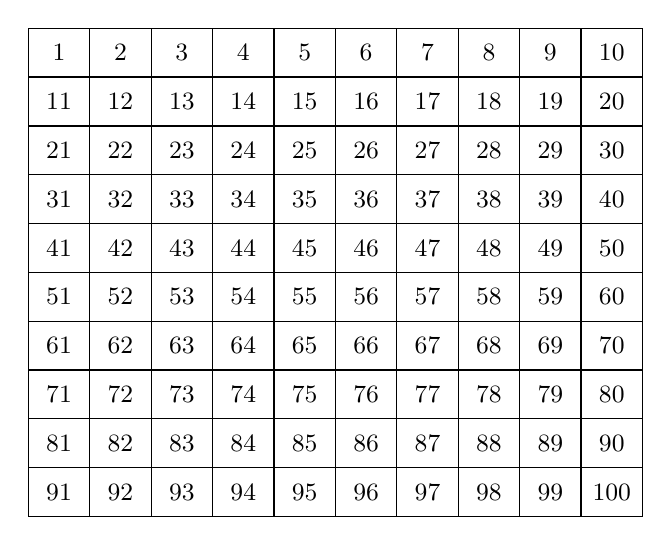
\begin{tikzpicture}[x=0.78cm,y=0.62cm]
  \foreach \n in {1,...,100}{
    \pgfmathtruncatemacro{\col}{mod(\n-1,10)}
    \pgfmathtruncatemacro{\lig}{9-floor((\n-1)/10)}
    \draw[line width=0.45pt] (\col,\lig) rectangle ++(1,1);
    \node[font=\small] at (\col+0.5,\lig+0.5) {\n};
  }
\end{tikzpicture}}

\begin{document}

\titreseq{Activité 6 -- Composer des bouquets identiques}

Un fleuriste dispose de :

\[
434\text{ roses}
\qquad\text{et}\qquad
620\text{ tulipes}.
\]

Il veut utiliser toutes les fleurs pour réaliser des bouquets
\textbf{tous identiques}, sans reste.

\section*{Partie A -- Comprendre la contrainte}

On note \(n\) le nombre de bouquets.

\begin{enumerate}
  \item Pourquoi \(n\) doit-il être un diviseur de \(434\) ?
  \item Pourquoi \(n\) doit-il aussi être un diviseur de \(620\) ?
  \item Que signifie alors « chercher toutes les possibilités » ?
\end{enumerate}

\lignesreponse{5}

\section*{Partie B -- Utiliser les facteurs premiers}

Décompose \(434\) et \(620\) en produits de facteurs premiers.

\[
434=\dotfill
\]

\[
620=\dotfill
\]

Quels facteurs apparaissent dans les deux décompositions ?

\lignesreponse{5}

\section*{Partie C -- Trouver tous les nombres de bouquets}

Dresse la liste de tous les diviseurs communs de \(434\) et \(620\).

\[
\dotfill
\]

Complète le tableau pour chacune des possibilités.

\renewcommand{\arraystretch}{1.55}
\begin{tabularx}{0.9\textwidth}{
|>{\centering\arraybackslash}X
|>{\centering\arraybackslash}X
|>{\centering\arraybackslash}X|}
\hline
\textbf{Nombre de bouquets} &
\textbf{Roses par bouquet} &
\textbf{Tulipes par bouquet}\\
\hline
& & \\
\hline
& & \\
\hline
& & \\
\hline
& & \\
\hline
\end{tabularx}

\section*{Partie D -- Interpréter}

\begin{enumerate}
  \item Quel est le plus grand nombre de bouquets possible ?
  \item Quelle est alors la composition de chaque bouquet ?
  \item Le fleuriste peut-il réaliser \(10\) bouquets ? Justifie.
  \item Le fleuriste peut-il réaliser \(31\) bouquets ? Justifie.
  \item Pourquoi la réponse « \(62\) bouquets » ne suffit-elle pas
        à la question demandant \textbf{toutes} les possibilités ?
\end{enumerate}

\lignesreponse{7}

\aretenir{Dans un problème de groupes identiques sans reste,
le nombre de groupes doit être un diviseur de chaque quantité.

En 4e, on peut chercher tous les diviseurs communs à l'aide
des décompositions en facteurs premiers, sans utiliser de formule de PGCD.}

\end{document}
